

\chapter{Datenaufbereitung}

Um die Deformation im eingespannten Zustand zu erkennen, muss das komplette Werkstück
als digitales Modell existieren, um es mit anderen Modellen vergleichen zu können.
Das Verfahren soll die Deformation nur in einer zweidimensionalen Perspektive erkennen. 
Das ist weniger komplex, hat aber zur Folge, dass Bauteile mit unterschiedlichen 
Oberflächenhöhen nicht korrekt analysiert werden können. 
Geometrie und Oberflächeninformationen des eingespannten Bauteils liegen 
in Form von mehreren Pointclouds vor.
Diese Daten wurden mithilfe eines Laserscanners aufgenommen. Durch diesen Prozess 
entstehen Messfehler und Ausreißer. Diese Punkte verfälschen das Verfahren da sie 
nicht auf dem eingespannte Bauteil liegen. Die Genauigkeit des Verfahrens profitiert, 
wenn diese Punkte entfernt werden.

\section{Pointcloud filtern} [TODO Komplett überarbeiten]

Wie in Abbildung \ref{fig:brightness} zu erkennen ist, streuen nicht alle Punktwolken
gleichmäßig. Abhängig vom Werkstoff des Bauteils reflektieren die Laserstrahlen 
unterschiedlich, was zu einer variierenden Anzahl von Ausreißern führt. 
Das Metallteil zeigt eine deutlich stärkere Streuung in beide Richtungen, 
während das FDM-gedruckte Bauteil weniger nach oben, 
aber mehr nach unten streut. Daher muss eine Filtermethode gewählt werden, 
die für alle Fertigungsverfahren anwendbar ist und nicht bei einem Verfahren 
besser funktioniert als bei einem anderen. Wird beispielsweise die Methode angewendet, 
die die 10 \% am häufigsten auftretenden Höhenwerte bei einem Metallteil berücksichtigt, 
ergibt sich das in Abbildung \ref{fig:metall_image} gezeigte Bild.
Man sieht vor allem auf der rechten Seite, dass Ränder nicht mehr klar erkennbar sind, 
da sie durch die Filterung Lücken aufweisen. Praxistests haben gezeigt das ein 
ausreichend gut funktionierender Filterwert 50 \% ist. Damit werden 
ausreichend viele Messfehler aus dem Bild genommen,
aber trotzdem bleiben Oberflächenstrukturen und Ränder
sichtbar, um ein korrektes Zusammenfügen zu gewährleisten.
Dieses Filtern bezieht sich aber nur auf zweidimensionale Bildinformationen.
Um bei dem Konvertieren noch weniger Punkte,
die nicht auf dem Bauteil liegen nicht in das Bild zu übernehmen, 
kann auch noch die Pointcloud gefiltert werden.
Hier kann ein einzelner Punkt relativ zu seinen Nachbarn im dreidimensionalen 
Raum betrachtet werden, um so Ausreißer zu erkennen. Dafür sind in der Open-Source
Bibliothek 'Open3D' zwei Methoden vorhanden: Radius basierte Entfernung,
oder auf Basis von statistischen Werten.
Die erste Methode eignet sich gut, wenn die Maße des Objekts bekannt
sind. Hier wird um jeden Punkt eine Kugel gebildet und alle Punkte die weniger als 
einen konfigurierbare Menge an Punkte in ihrer Kugel haben werden entfernt. Da 
das hier zu entwickelnde Verfahren sich nicht auf eine Bauteilgeometrie beschränken
ist dieses Verfahren nicht geeignet. Stattdessen wird das statistische genutzt. 
Hier werden alle Punkte entfernt die weiter von ihren benachbarten Punkten entfernt
sind als der durchschnittliche Abstand der Punkte in der gesamten Pointcloud. 
Hier kann die Menge der benachbarten Punkte die betrachtet werden sollen und
ein Limit für den Abstand von der Standardabweichung. 
Umso mehr benachbarte Punkte betrachtet werden, desto länger dauert der Filterprozess, 
aber die Filterung wird auch akkurater. Im Praxistest haben sich
hier 50 Nachbarpunkte bewährt. Mit diesem Wert werden bei Pointclouds in unserem 
Datensatz jeweils ca. zwei Prozent aller Punkte entfernt. So kann das resultierende
Bild ausreichend gut umgewandelt werden, um eine erfolgreiche Zusammenführung 
von verschiedenen Bildern zu gewährleisten.
Ein Nachteil bei der Filterung in Abbildung \ref{fig:image_from_pc} links und rechts 
mittig zu sehen. Hier sind schwarze Punkte sichtbar. Diese treten auf, weil der Scanner
hier über dem Bauteil Punkte erkannt hat. Durch das Filtern wurden diese Punkte entfernt
beziehungsweise bei der Konvertierung nicht berücksichtigt. Da diese Punkte dann fehlen
bleiben sie im resultierenden Bild schwarz.

\section{Pointcloud in Bild konvertieren}

Um Rechenzeit zu sparen und die zahlreichen Funktionen bereits bestehender
 Bilderkennungsbibliotheken nutzen zu können, wurden die Punktwolken in Bilder 
 konvertiert. Hierfür wird zunächst ein leeres Bild mit den gleichen 
 Maßen der Pointcloud erstellt. Anschließend wird über alle Punkte der
 Pointcloud iteriert und der Pixel an den 
 entsprechenden X- und Y-Koordinaten des Punktes auf einen Helligkeitswert gesetzt.

Um Rechenzeit und Speicherkapazitäten zu schonen und 
da es für die Berechnungen ausreichend ist, wurden 
8-Bit-Single-Channel-Bilder verwendet, die nur Helligkeitswerte abbilden. 
In diesen Bildern kann jeder Pixel einen Wert zwischen 0 und 255 annehmen. 
Der entsprechende Helligkeitswert kann wie folgt berechnet werden:
\begin{align}\label{calc:brightness}
    value_p = \frac{Z - min_z}{max_z - min_z} \cdot (max_{brightness} - min_{brightness}) + min_{brightness}
\end{align}
Der resultierende Wert ist die Helligkeit, die dem Pixel zugewiesen wird.
$Z$ ist die Z-Koordinate des Punktes in der Pointcloud. $min_y$ und $max_y$ sind 
die Grenzen der Z-Koordinate, diese werden gebraucht um die Helligkeit relativ 
zu der Höhe zu berechnen. $min_{brightness}$ und $max_{brightness}$ sind die gewünschten Grenzen der 
Helligkeit. In unserem Fall sind $min_{brightness} = 0$ und $max_{brightness} = 255$ da ein 8 Bit Bild
verwendet wird.


\begin{figure}[H]
    \centering
    \begin{minipage}{0.45\textwidth}
        \centering
        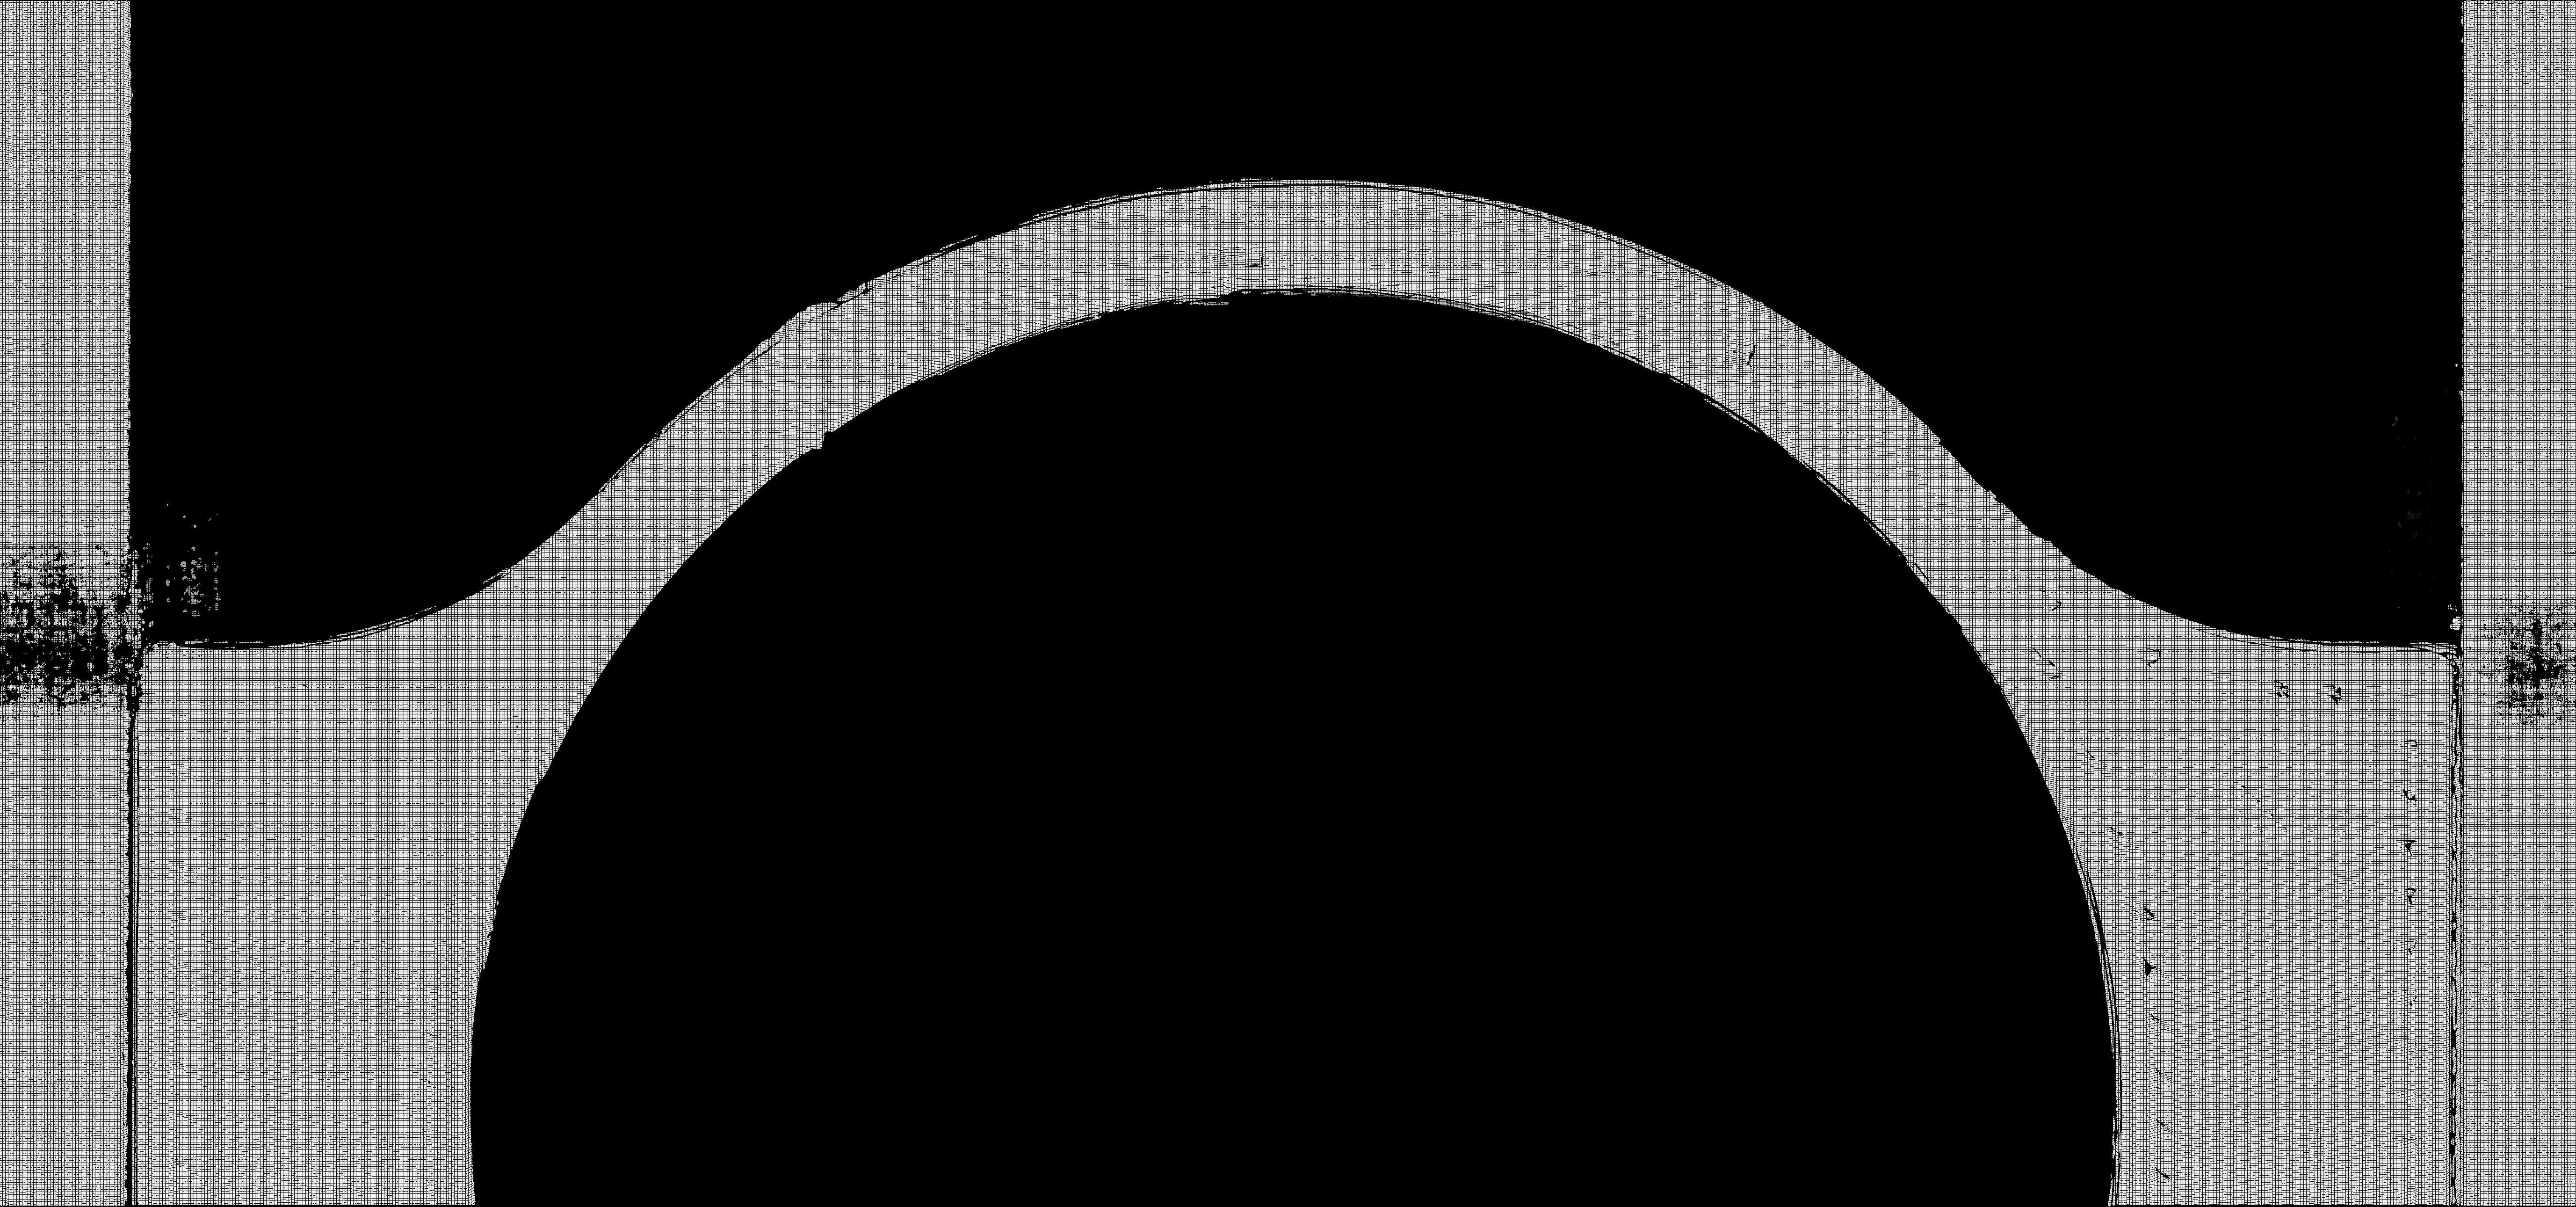
\includegraphics[width=0.98\textwidth]{images/fdm_top_100p.png} % first figure itself
        \caption*{(a)}
    \end{minipage}\hfill
    \begin{minipage}{0.45\textwidth}
        \centering
        \includegraphics[width=0.98\textwidth]{images/fdm_top_10p.png} % second figure itself
        \caption*{(b)}
    \end{minipage}
    \caption{Resultat der Pointcloud zu Bild Konvertierung. (a) Ohne Filterung der Höhenwerte, (b) Die gleichen 
    Scandaten, aber nur den zehn Prozent häufigsten Höhenwerten.}
    \label{fig:image_from_pc}
\end{figure}

Wie man in Abbildung \ref{fig:image_from_pc} sehen kann, sind kaum Helligkeitsveränderungen
im Bild sichtbar. Das liegt an derselben Problematik, an der der ICP-Algorithmus \ref{icp} häufig
scheitert. Reale Datensets spiegeln die Realität nicht ganzheitlich korrekt wider, sondern
beinhalten Messfehler und Streuungen.

\begin{figure}[H]
    \centering
    \begin{minipage}{\textwidth}
        \centering
        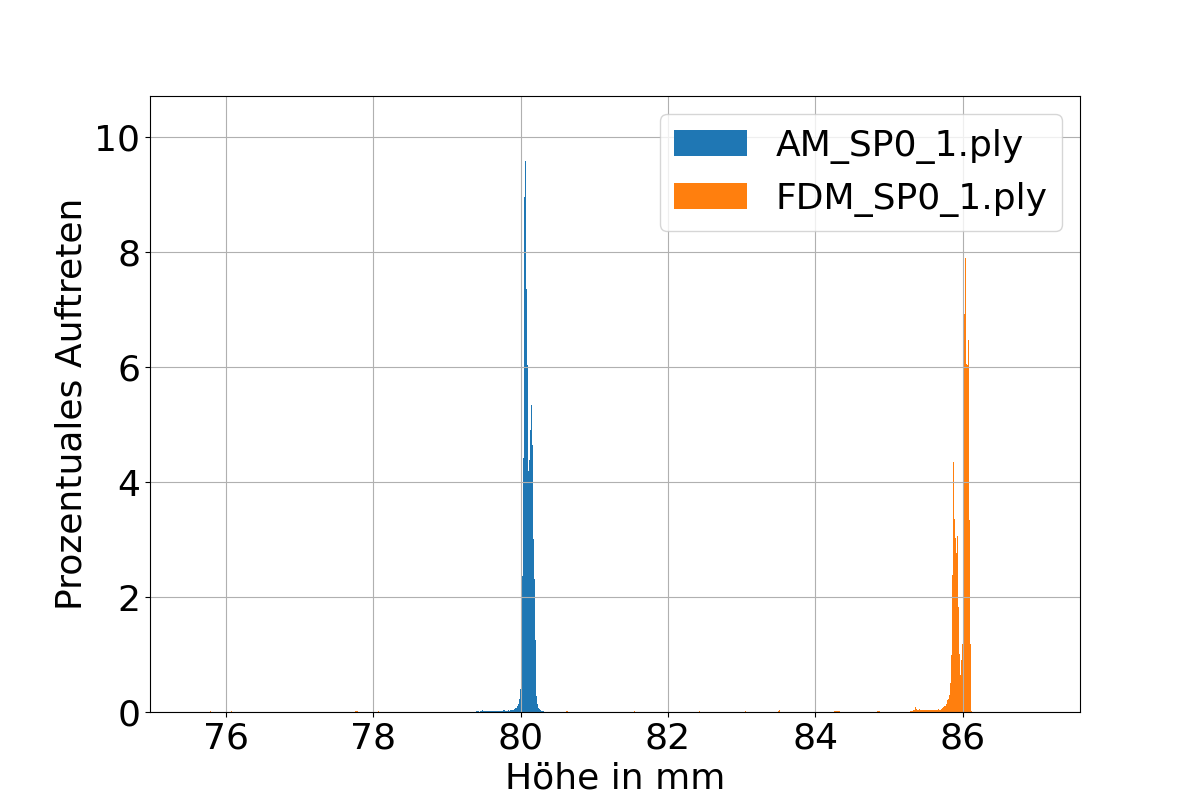
\includegraphics[width=0.8\textwidth]{images/height_occurange.png} % first figure itself
        \caption*{(a)}
    \end{minipage}\hfill
    \begin{minipage}{\textwidth}
        \centering
        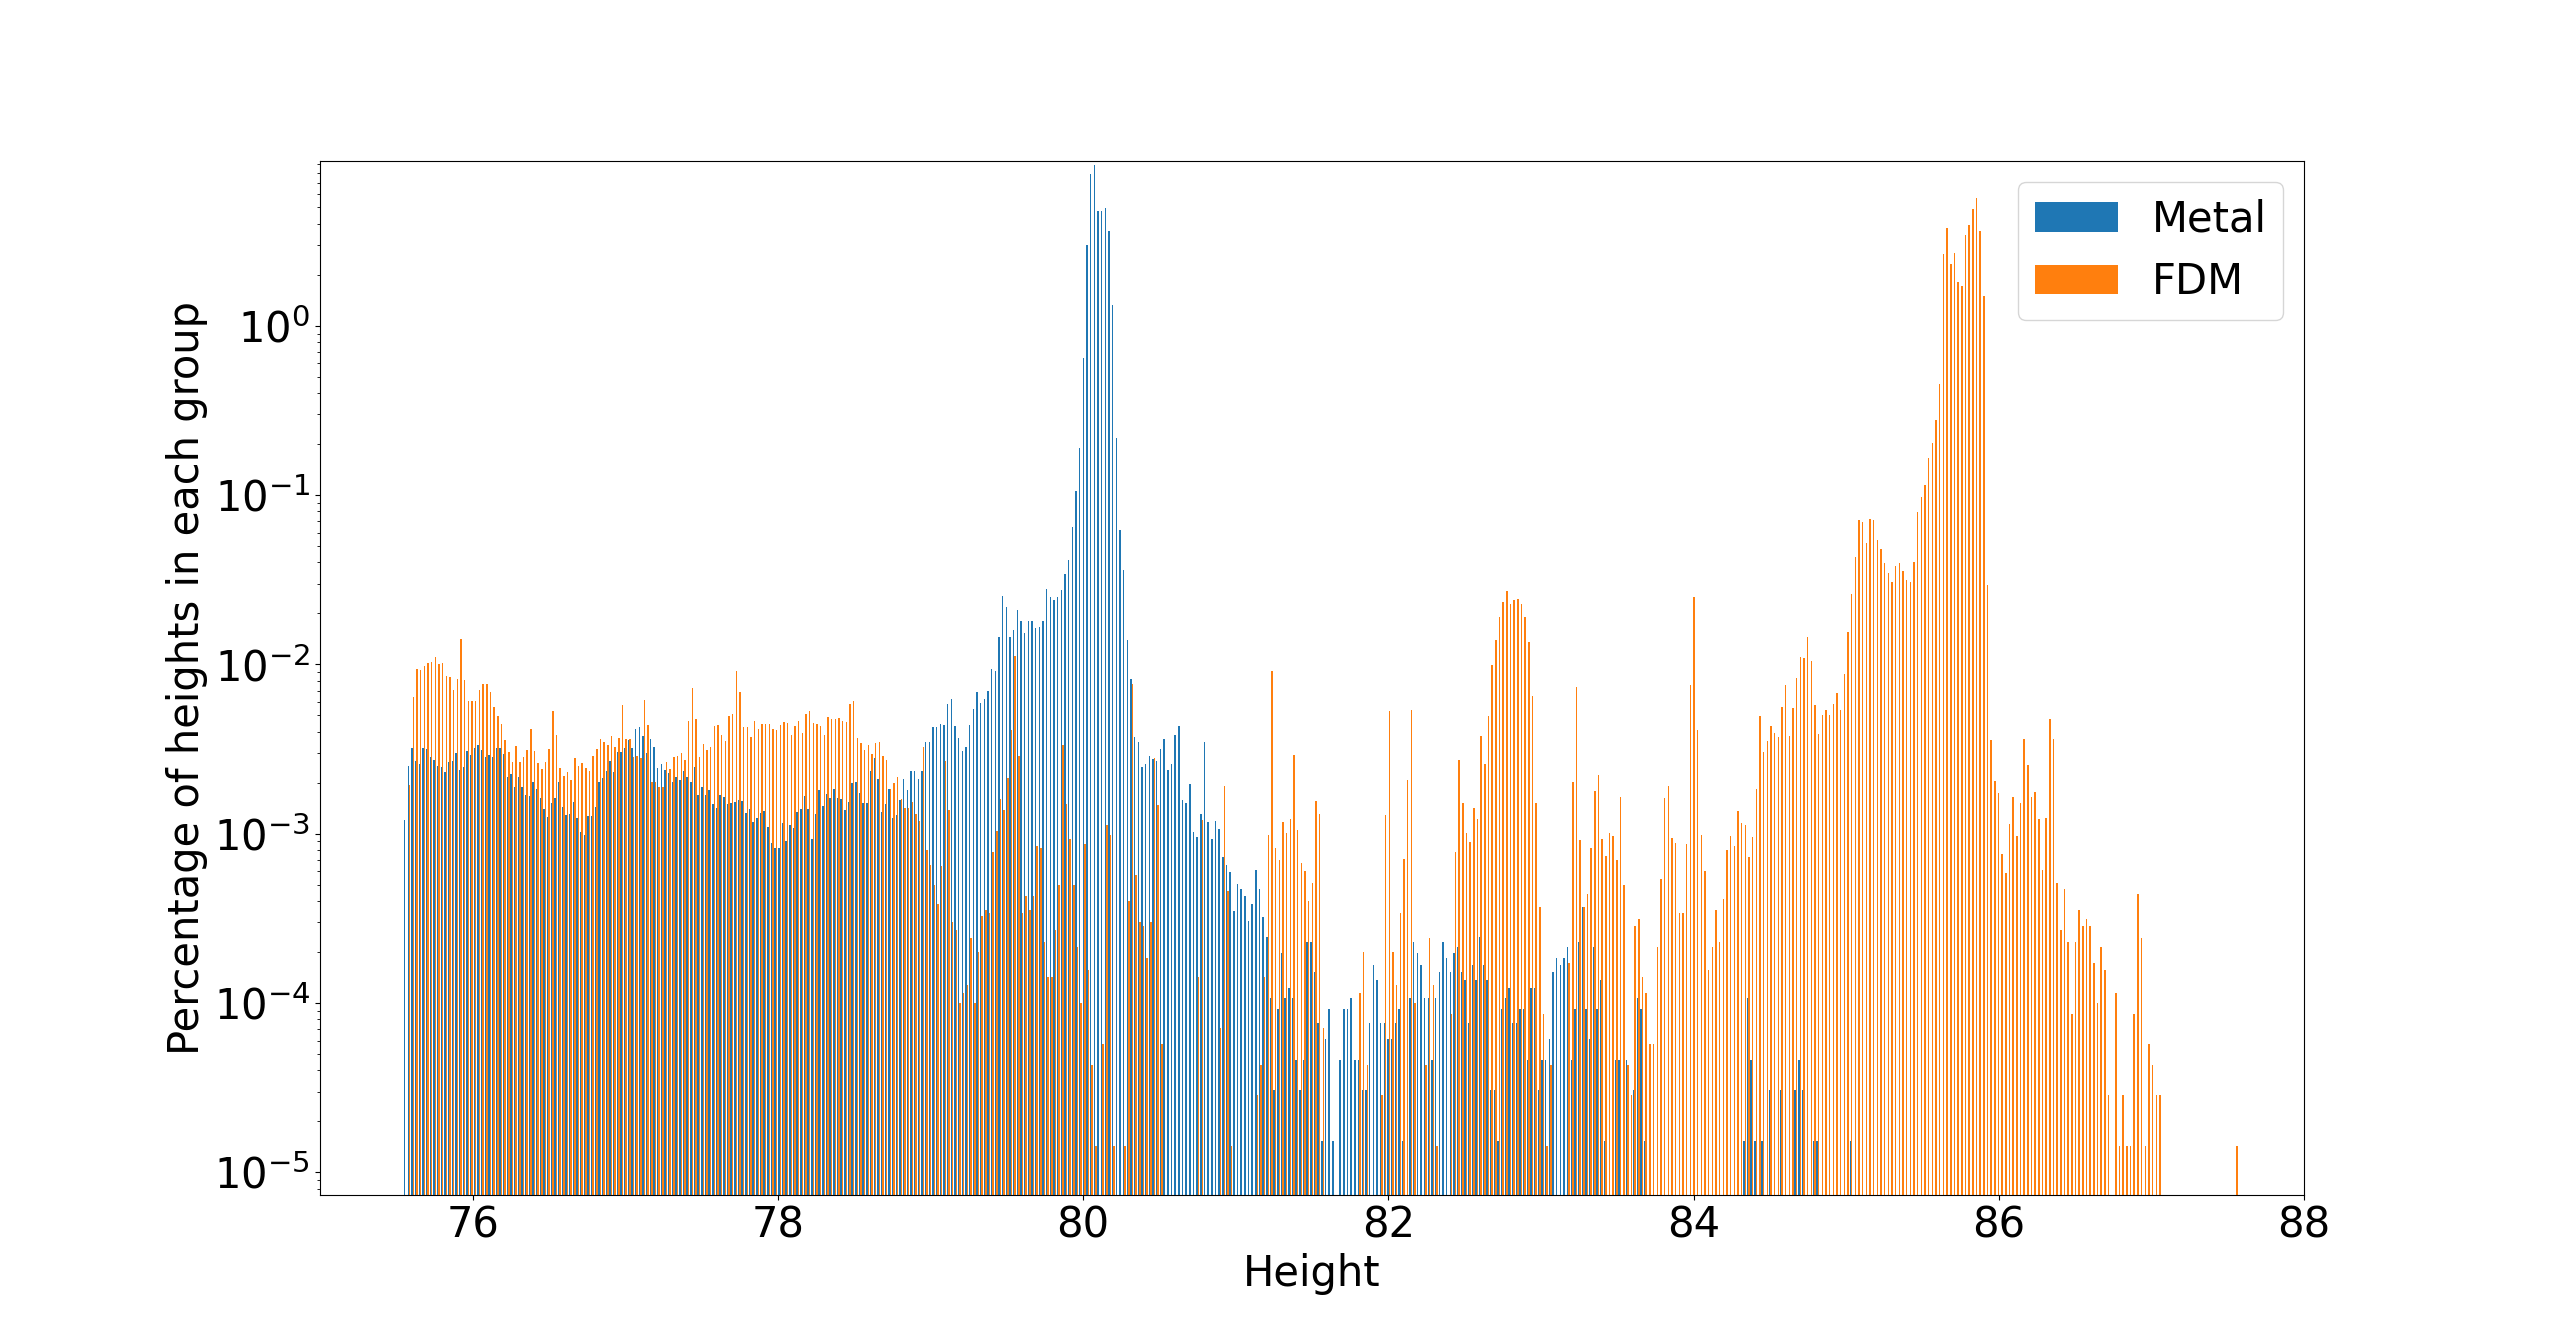
\includegraphics[width=0.8\textwidth]{images/height_occurange_log.png} % second figure itself
        \caption*{(b)}
    \end{minipage}
    \caption{Auftreten der Höhenwerte in den Scandaten der Demonstratorbauteile. 
    (a): Das Histogramm ist nicht skaliert. (b): Logarithmische Skalierung der 
    Höheninformationen. Hier ist zu sehen das viele kleine Werte vorliegen.}
    \label{fig:brightness}
\end{figure}


\begin{figure}
    \centering
    \includegraphics[width=0.8\textwidth]{images/am_sp0_top_10p.png}
    \caption{Metallteil gefiltert}
    \label{fig:metall_image}
\end{figure}

Abbildung \ref*{fig:brightness} zeigt die Häufigkeit der gleichen Höhenwerte einer
Pointcloud von dem Demonstratorbauteil [TODO Erklärung Demonstratorbauteil]. In blau ist die Verteilung der Punkte auf 
einem Demonstratorbauteil zu sehen, das aus Metall gedruckt wurde, orange zeigt die 
Verteilung der Punkte auf einem Kunststoffteil.
In dem oberen Histogramm 
sind die Häufigkeiten der Höhenwerte zu sehen. Der Datensatz wurde in 500 gleich große
Teile gruppiert, jeder Balken repräsentiert eine Gruppe.
Unterhalb ist das Histogramm mit dem gleichen Datensatz, aber mit der y-Achse 
logarithmisch skaliert um kleine Prozente deutlich zu machen die im
oberen Diagramm nur schwer oder gar nicht sichtbar sind. 
Die meisten Höhenwerte treten bei ca. 80 mm beziehungsweise 85 mm auf, 
sie gehören zu den Punkten, die auf dem Demonstratorbauteil liegen, 
es treten allerdings auch Werte darunter und darüber auf. 
Die in \ref*{calc:brightness} vorgestellte Formel benutzt allerdings 
die absoluten Minimum und Maximum Werte.
Alle Punkte die tatsächlich auf dem Bauteil werden also entsprechend wenig
berücksichtigt. Dies kann verhindert werden, indem Werte, die weniger häufig 
auftreten, entfernt werden. Sortiert man alle Höhenwerte nach der Häufigkeit ihres 
Auftretens in der Pointcloud und entfernt den n-ten Prozentsatz können Ausreißer 
entfernt werden. Wenn nur die häufigsten zehn Prozent übernommen werden erhält man 
das untere Bild in Abbildung \ref{fig:image_from_pc}

Ränder und Oberflächenstrukturen auf dem Bauteil können jetzt deutlich besser erkannt werden. Auch zu sehen
sind jetzt die Markierungen auf der linken und rechten Seite, die bei der Registrierung
helfen sollen. Zusätzlich sind die Spuren und Lücken die durch den FDM 
Herstellungsprozess entstehen zu sehen.

Durch das Filtern der Höheninformationen sind Oberflächenstrukturen nicht nur besser
erkennbar, auch die Ränder treten genauer hervor. 
Dadurch können die Bilder im weiteren Schritt korrekt zusammengefügt werden

